\documentclass[11pt]{article}
\usepackage{amsmath, amssymb, amscd, amsthm, amsfonts}
\usepackage[a4paper]{geometry}
\usepackage{graphicx}
\graphicspath{ {./images/} }
\usepackage{hyperref}
\usepackage[italian]{babel}
\usepackage{tikz}
\usetikzlibrary{shapes, arrows.meta, positioning}

\oddsidemargin 0pt
\evensidemargin 0pt
\marginparwidth 40pt
\marginparsep 10pt
\topmargin -20pt
\headsep 10pt
\textheight 8.7in
\textwidth 6.65in
\linespread{1.2}

\title{Piattaforma di Gough-Stewart}
\author{Daniele Facco}
\date{}

\newtheorem{theorem}{Theorem}
\newtheorem{lemma}[theorem]{Lemma}
\newtheorem{conjecture}[theorem]{Conjecture}

\newcommand{\rr}{\mathbb{R}}

\newcommand{\al}{\alpha}
\DeclareMathOperator{\conv}{conv}
\DeclareMathOperator{\aff}{aff}

\begin{document}

\maketitle
\tableofcontents
\newpage

\begin{abstract}
Studio della piattaforma di Stewart e dei suoi componenti.
\end{abstract}

\section{Servomotori}\label{servomotori}
I servomotori sono l'elemento principale nella realizzazione della piattaforma di Stewart.

\begin{figure}[h!]
\centering
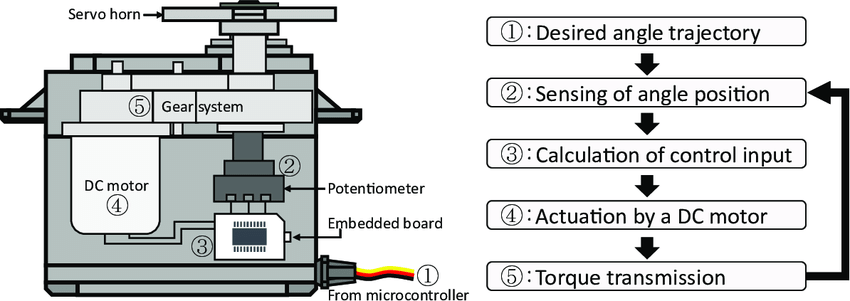
\includegraphics[scale=0.3]{Schematic-of-an-RC-servo-motor.png}
\end{figure}

Questi motori sono controllati in modalità PWM dalla scheda Arduino tramite un'apposita libreria. Il segnale inviato ai servomotori è periodico, di periodo 20ms e presenta uno stato on/off a livello logico per un tempo prefissato a seconda della posizione richiesta; ad esempio la posizione 0° prevede un livello logico alto di 1ms, 90° di 1,5ms e 180° di 2ms.

Il controllo di questi elementi è gestito dalla scheda Arduino tramite uno shield che ne facilita l'installazione. Una nota particolare va fatta in merito alla potenza richiesta dai servomotori, nonostante il loro consumo in stato 'idle' sia di circa 10mW, durante il movimento questo può raggiungere oltre 300mW. É quindi necessaria una alimentazione esterna che sia in grado di fornire almeno 2A a 5V in quanto la scheda alimentata, tramite usb dalla presa del computer, può ricevere al massimo 1A.

\section{Piattaforma di Stewart}\label{piattaformastewart}
La piattaforma di Stewart è un particolare sistema meccanico, costituito da una base su cui sono posizionati 6 attuatori di vario tipo collegati alla piattaforma superiore mediante giunti snodabili. Un esempio comune sono gli attuatori prismatici: pistoni lineari che presentano un solo grado di libertà. Nel progetto vengono impiegati servomotori che presentano il vantaggio di essere certamente più economici rispetto agli attuatori prismatici ma il sistema risultante assume un grado di complessità superiore. Tramite opportune osservazioni matematiche è possibile risalire ad un modello equivalente a quello degli attuatori prismatici che garantisce un range di movimento ottimale.

\section{Robot seriali e paralleli}\label{robotserialiparalleli}
È utile enunciare la differenza tra robot di tipo seriale e parallelo per comprendere le successive implicazioni a livello matematico.
I robot seriali prevedono una serie di giunti snodabili controllati da attuatori, che spesso assumono le caratteristiche di un arto antropomorfo. 
Questi tipi di robot prendono spesso il nome di braccio meccanico e trovano ampia applicazione nell'industria meccanica.
Nei robot paralleli invece, gli attuatori agiscono tutti sullo stesso elemento tramite giunti indipendenti. 
La piattaforma di Stewart ne è il principale esempio e trova applicazione soprattutto nella realizzazione di simulatori avanzati di volo o per testare veicoli nelle case automobilistiche.
Entrambi i sistemi presentano 6 gradi di libertà, indicati anche come 6DOF, ma il problema matematico che li caratterizza è fondamentalmente opposto.


\section{Cinematica diretta e inversa}\label{cinematicadirettainversa}

\newpage
\section{Analisi della piattaforma di Stewart con attuatori rotativi}\label{analisi}

Il problema della piattaforma di Stewart controllata da attuatori rotativi è fondamentalmente costituito da due sottoproblemi.
Uno relativo alla determinazione delle lunghezze dei vettori che collegano la base alla piattaforma per ogni possibile posizione e l'altro relativo all'implementazione stessa dei servomotori, per via della complessità di descrizione del sistema biella manovella impiegato. 

\subsection{Analisi problema piattaforma}

Si definiscono due sistemi di riferimento cartesiani che caratterizzano il sistema, mostrati nella figura \ref{fig:rv}, uno fisso per la base centrato in $O$ di versori $\hat{i},\hat{j},\hat{k}$ e uno variabile per la piattaforma centrato in $O'$ di versori $\hat{i'},\hat{j'},\hat{k'}$. Sono note le coordinate in tre dimensioni dei punti degli assi di rotazione dei servomotori $({B_i})$ e dei giunti della piattaforma $(P_i)$, quando questa è in posizione orizzontale a riposo rispetto al sistema di riferimento centrato nella base. Il problema consiste nel definire la posizione dei giunti della piattaforma nello spazio al variare di un set di valori $(x,y,z,\varphi,\vartheta,\psi)$ rispetto al riferimento fisso della base. I valori $(x,y,z,\varphi,\vartheta,\psi)$ precedentemente enunciati, si riferiscono alla posizione e rotazione nello spazio della piattaforma rispetto alla base; $(x,y,z)$ sono i valori del centro della piattaforma mentre $(\varphi,\vartheta,\psi)$ sono le rotazioni, rispettivamente roll, pitch e yaw (rollio, beccheggio e imbardata). Nell'analisi, si considerano separatamente gli effetti traslativi e rotativi.

\begin{figure}[h!]
\centering

\scalebox{0.83}{
\begin{tikzpicture}

\filldraw[fill=yellow!50,rotate around={-10:(0,7cm)},xshift=2cm,yshift=1cm] (0,7cm) ellipse (4cm and 2cm);
\filldraw [fill=red!50](0,0) ellipse (5cm and 2.5cm);
\draw [-latex, thick] (0,0) -- node[anchor=south]{$\hat b_i$}(5cm,0);
\draw [-latex, thick] (0,0) -- node[anchor=east]{$\hat T$}(2.15cm,7.65cm);
\draw [-latex, thick] (0,0) -- node[anchor=north]{$\hat q_i$}(6.1cm,6.95cm);
\draw [-latex, thick] (5cm,0) -- node[anchor=west]{$\hat l_i$}(6.1cm,6.95cm);
\draw[-latex, thick,rotate around={-10:(0,7cm)},xshift=2cm,yshift=1cm] (0cm,7cm) -- node[anchor=south]{$\hat p_i$}(4cm,7cm);
\filldraw [fill=black] (0,0) circle (2pt) node[yshift= -0.25cm] {$O$} node[xshift= -2cm] {Base};
\filldraw [fill=black] (5cm,0) circle (2pt) node[anchor=west]{$B_i$};
\filldraw [fill=black] (2.15cm,7.65cm) circle (2pt) node[yshift= 0.25cm] {$O'$} node[xshift= -2cm] {Piattaforma};
\filldraw [fill=black] (6.1cm,6.95cm) circle (2pt) node[anchor=west]{$P_i$};
\draw [-latex, thick] (-1,-1.5) -- node[anchor=north]{$\hat i$}(0cm,-1.5cm);
\draw [-latex, thick] (-1,-1.5) -- node[anchor=east]{$\hat k$}(-1cm,-0.5cm);
\draw [-latex, thick,rotate around={-120:(-1,-1.5cm)}] (-1,-1.5) -- node[anchor=east]{$\hat j$}(-0.5cm,-1.5cm);

\draw [-latex, thick,rotate around={-10:(0,8.5cm)}] (0,8.5) -- node[anchor=north]{$\hat {i'}$}(1cm,8.5cm);
\draw [-latex, thick,rotate around={-10:(0,8.5cm)}] (0,8.5) -- node[anchor=east]{$\hat {k'}$}(0cm,9.5cm);
\draw [-latex, thick,rotate around={-130:(0,8.5cm)}] (0,8.5) -- node[anchor=east]{$\hat {j'}$}(0.5cm,8.5cm);

\end{tikzpicture}
}
\caption{Sistemi di rifermento e vettori nel piano di Stewart.} \label{fig:rv}
\end{figure}

\subsubsection{Analisi traslazione $(x,y,z)$}\label{xyz}
Le variazioni in $(x,y,z)$ comportano una semplice traslazione dei punti del piano, questa viene indicata con un vettore $\hat T$ che adrà poi a sommarsi alla variazione dovuta a $(\varphi,\vartheta,\psi)$.

\subsubsection{Analisi rotazione $(\varphi,\vartheta,\psi)$}\label{ftp}
Per semplificare l'analisi si considerano, separatamente, gli effetti dovuti a queste tre componenti. Si studia il caso di solo rollio $(\varphi,0,0)$ per risalire alle coordinate di un punto $P$ rispetto alla base in seguito a una rotazione di $\varphi$ gradi. Per fare ciò, è necessario ottenere un'applicazione lineare che permetta di passare dal sistema di coordinate della piattaforma al sistema di coordinate della base.

% INSERIRE DISEGNO CAMBIO COORDINATE

Dallo studio della variazione troviamo che:

\begin{equation}\label{sistema1}
\begin{cases} 
x=x' \\ 
y=OA-CB=y'cos(\varphi)-z'sin(\varphi) \\ 
z=AB+CP=y'sin(\varphi)-z'cos(\varphi)
\end{cases} 
\end{equation}


Per comodità di calcolo nei successivi passaggi il sistema \eqref{sistema1} viene riscritto in forma matriciale.

\begin{equation}\label{rx}
R_x(\varphi)=
\begin{bmatrix}
1 & 0 & 0\\
0 & cos(\varphi) & -sin(\varphi)\\
0 & sin(\varphi) & cos(\varphi)
\end{bmatrix}
\quad : \quad
\begin{bmatrix}
x \\
y \\
z 
\end{bmatrix}
=R_x(\varphi)\cdot\begin{bmatrix}
x' \\
y' \\
z' 
\end{bmatrix}
\end{equation}
Risultati analoghi si ottengono per $\vartheta$ e $\psi$:
\begin{equation}\label{ry}
R_y(\vartheta)=
\begin{bmatrix}
cos(\vartheta) & 0 & sin(\vartheta)\\
0 & 1 & 0\\
-sin(\vartheta) & 0 & cos(\vartheta)
\end{bmatrix}
\end{equation}
\begin{equation}\label{rz}
R_z(\psi)=
\begin{bmatrix}
cos(\psi) & -sin(\psi) & 0\\
sin(\psi) & cos(\psi) & 0\\
0 & 0 & 1\\
\end{bmatrix}
\end{equation}

Le singole matrici possono essere viste come applicazioni lineari, si procede quindi nella moltiplicazione di \eqref{rx}, \eqref{ry} e \eqref{rz} per ottenere una singola applicazione lineare composta. Notare che nel prodotto tra matrici non vale la proprietà commutativa, bisongna quindi valutare attentamente l'ordine di moltiplicazione, altrimenti si otterrà una rotazione erronea. I passaggi intermedi vengono ommessi in quanto ripetono tre volte una semplice operazione di moltiplicazione tra matrici.
\begin{align}\label{rg}
    R_g &= R_z(\psi)\cdot R_y(\vartheta)\cdot R_x(\varphi)\\
    		&= \begin{bmatrix}
			cos(\vartheta)cos(\psi) & -cos(\varphi)sin(\psi)+sin(\varphi)sin(\vartheta)cos(\psi) & sin(\varphi)sin(\psi)+cos(\varphi)sin(\vartheta)cos(\psi)\\
			cos(\vartheta)sin(\psi) & cos(\varphi)cos(\psi)+sin(\varphi)sin(\vartheta)sin(\psi) & -sin(\varphi)cos(\psi)+cos(\varphi)sin(\vartheta)sin(\psi)\\
			-sin(\vartheta) & sin(\varphi)cos(\vartheta) & cos(\varphi)cos(\vartheta)
			\end{bmatrix}
\end{align}

Moltiplicando il vettore $\hat{p_i}$ per la matrice di rotazione \eqref{rg} si ottengono le coordinate del punto $P_i$ nel sistema di riferimento della base. 

\subsubsection{Conclusione problema piattaforma}
Grazie ai risultati ottenuti nelle sezioni \ref{xyz} e \ref{ftp} si possono definire i vettori $\hat{q_i}$ che descrivono la posizione dei punti $P_i$ rispetto al centro del sistema di riferimento della base $O$ per ogni operazione rototraslativa.
\begin{equation}\label{qi}
\hat{q_i}=\hat{T}+R_g\cdot \hat{p_i}
\end{equation}
Una volta ottenuto questo vettore, con una semplice operazione vettoriale, si può risalire a $\hat{l_i}$, vettore che descrive la distanza tra l'asse del servomotore e il corrispettivo giunto sulla piattaforma.

\begin{align}\label{li}
\hat{l_i}=\hat{T}+R_g\cdot \hat{p_i}-\hat{b_i}
\end{align}
Nel caso della piattaforma di Stewart, sei equazioni \eqref{li} permettono di descrivere la posizione della piattaforma al variare di $(x,y,z,\varphi,\vartheta,\psi)$.
Notare come con l'impiego di attuatori lineari, il problema si risolve assegnando queste lunghezze per ottenere la posizione desiderata. 

\subsection{Analisi problema attuatori rotativi}
L'impiego di servomotori complica ulteriormente le equazioni, è infatti necessario un numero di variabili superiore per descrivere in modo appropriato il sistema. Ogni servomotore controllando un giunto biella manovella collegato alla piattaforma regola la lunghezza del vettore $\hat{l_i}$. Si rende quindi fondamentale trovare una relazione tra l'angolo del servomotore e il vettore $\hat{l_i}$. Anche in questo caso il problema può essere separato in due parti: la determinazione della posizione del giunto biella manovella e la ricerca dell'angolo di rotazione $\alpha$.

\begin{figure}[h!]
\centering
\scalebox{0.67}{
\begin{tikzpicture}
\filldraw [fill=blue!50](0,0) rectangle (2,4);
\filldraw [fill=black] (1cm,3cm) circle (10pt);
\draw [line width=2pt] (1cm,3cm) -- node[anchor=east, xshift= 0.6cm,yshift=-0.45cm]{$m$}(3cm,2cm);
\filldraw [fill=black] (3cm,2cm) circle (3pt);
\filldraw [fill=black] (2cm,9cm) circle (3pt);
\draw [line width=2pt] (3cm,2cm) -- node[anchor=west]{$b$}(2cm,9cm);
\draw [line width=2pt,dashed] (1cm,3cm) -- node[anchor=east]{$l$}(2cm,9cm);
%\draw [<->] (3.5cm,2.2cm) arc (150:125:33.7pt);
\end{tikzpicture}
}
\caption{Sistema biella manovella con i servomotori.} \label{fig:rv}
\end{figure}

\subsubsection{Posizione del giunto biella manovella}
Note le lunghezze della biella $b$ e della manovella $m$, si valuta l'angolo di inclinazione dei servomotori rispetto all'asse $x$ e si indica con $\beta$, e si nota come i servomotori siano a due a due specchiati. Due set di equazioni saranno quindi necessarie per descrivere i motori pari e dispari al variare di $\alpha$.
\begin{equation}\label{bmpari}
    \begin{cases}
      x_{bm}=m \cdot cos(\alpha)cos(\beta)+x_b\\
      y_{bm}=m \cdot cos(\alpha)sin(\beta)+y_b\\
      z_{bm}=m \cdot sin(\alpha)+z_b\\
    \end{cases}\quad pari
\end{equation}
\begin{equation}\label{bmdispari}
    \begin{cases}
      x_{bm}=m \cdot cos(\alpha)cos(\pi+\beta)+x_b\\
      y_{bm}=m \cdot cos(\alpha)sin(\pi+\beta)+y_b\\
      z_{bm}=m \cdot sin(\alpha)+z_b\\
    \end{cases}\quad dispari
\end{equation}
Applicando le nozioni trigonometriche: 
$$cos(\alpha)=-cos(\alpha) \quad cos(\pi+\beta)=-cos(\beta) \quad sin(\pi+\beta)=-sin(\beta)$$
ai sistemi \eqref{bmpari} e \eqref{bmdispari} risulta evidente che questi due sono equivalenti.
\subsubsection{Determinazione angolo $\alpha$}
Per la determinazione dell'angolo $\alpha$ ottimale esistono due tecniche principali. La prima consiste in una ricerca binaria (o dicotomica) del valore che meglio soddisfa le equazioni della posizione. La seconda prevede un approccio matematico più estensivo per determinare il valore \textbf{esatto} di $\alpha$ in base ad una $l$ fornita. Il primo approccio risulta più semplice dal punto di vista realizzativo ma a suo discapito è poco efficiente, in quanto richiede un numero arbitrario di iterazioni per raggiungere una determinata precisione di $\alpha$. Il secondo è invece più difficile da ottenere a causa dei calcoli non del tutto intuitivi ma garantisce di raggiungere la soluzione ottimale con una sola computazione. Per lo svolgimento del progetto è stata impiegata la seconda opzione.

Per il teorema di Pitagora in tre dimensioni abbiamo che:
\begin{align}\label{m2}
    m^2 &= (x_{bm}-x_b)^2+(y_{bm}-y_b)^2+(z_{bm}-z_b)^2\\
    		&= (x_{bm}^2+y_{bm}^2+z_{bm}^2)+(x_{b}^2+y_{b}^2+z_{b}^2)-2(x_{bm}x_b+y_{bm}y_b+z_{bm}z_b)
\end{align}
\begin{align}\label{l2}
    l^2 &= (x_{q}-x_b)^2+(y_{q}-y_b)^2+(z_{q}-z_b)^2\\
    		&= (x_{q}^2+y_{q}^2+z_{q}^2)+(x_{b}^2+y_{b}^2+z_{b}^2)-2(x_{q}x_b+y_{q}y_b+z_{q}z_b)
\end{align}
\begin{align}\label{b2}
    b^2 &= (x_{q}-x_{bm})^2+(y_{q}-y_{bm})^2+(z_{q}-z_{bm})^2\\
    		&= (x_{q}^2+y_{q}^2+z_{q}^2)+(x_{bm}^2+y_{bm}^2+z_{bm}^2)-2(x_{q}x_{bm}+y_{q}y_{bm}+z_{q}z_{bm})
\end{align}

I valori di $m^2$, $l^2$ e $b^2$ sono noti, si sostituiscono le equazioni \eqref{m2} e \eqref{l2} in \eqref{b2}, si ottiene:
\begin{align}\label{passaggio}
    l^2-(b^2-m^2) =& 2(x_{b}^2+y_{b}^2+z_{b}^2)+2x_{bm}(x_q-x_b)+2y_{bm}(y_q-y_b)+2z_{bm}(z_q-z_b)\\ 
    				   & -2(x_qx_b+y_qy_b+z_qz_b)
\end{align}

Si sostituiscono le equazioni dei valori noti $x_{bm}$, $y_{bm}$ e $z_{bm}$ calcolate in \eqref{bmpari} e si svolgono le dovute semplificazioni.
\begin{align}\label{passaggio}
    l^2-(b^2-m^2) =& 2(x_{b}^2+y_{b}^2+z_{b}^2)+2[m \cdot cos(\alpha)cos(\beta)+x_b](x_q-x_b)\\
    &+2[m \cdot cos(\alpha)sin(\beta)+y_b](y_q-y_b)+2[m \cdot sin(\alpha)+z_b](z_q-z_b)\\ 
    				   & -2(x_qx_b+y_qy_b+z_qz_b)\\
    				   =& 2m \cdot cos(\alpha)cos(\beta)(x_q-x_b)+2m \cdot cos(\alpha)sin(\beta)(y_q-y_b)\\
    				   & +2m \cdot sin(\alpha)(z_q-z_b)\\
    				   =& 2m \cdot sin(\alpha)(z_q-z_b) +2m \cdot cos(\alpha)[cos(\beta)(x_q-x_b)+sin(\beta)(y_q-y_b)]   
\end{align}

L'equazione \eqref{passaggio} è nella forma $L=Mcos(\alpha)+Nsin(\alpha)$ e può essere ulteriormente compattata considerando la formula della somma di segnali sinusoidali di ampiezza diversa, secondo la quale un segnale $Acos(\alpha)+Bsin(\alpha)$ può essere riscritto come $Csin(\alpha + \nu)$, infatti:
\begin{equation}\label{c}
Csin(\alpha + \nu)=Csin(\alpha)\cdot cos(\nu)+Ccos(\alpha)\cdot sin(\nu)
\end{equation}
\begin{equation}\label{tg}
    \begin{cases}
      A=Ccos(\nu)\\
      B=Csin(\nu)\\
    \end{cases}\quad \Rightarrow \quad  C=\sqrt{A^2+B^2}, \quad \nu=arctan\left(\frac{B}{A}\right)
\end{equation}

Applicando il risultato ottenuto in \eqref{tg} possiamo quindi scrivere:
\begin{align}\label{alfa}
    L= \sqrt{M^2+N^2}\cdot sin\left(\alpha+arctan\left(\frac{N}{M}\right)\right) \quad  &\Rightarrow\\ sin\left(\alpha+arctan\left(\frac{N}{M}\right)\right)=\frac{L}{\sqrt{M^2+N^2}}  \quad  &\Rightarrow\\
    \alpha=arsin\left(\frac{L}{\sqrt{M^2+N^2}}\right)-arctan\left(\frac{N}{M}\right)
\end{align}
Con rispettivamente:
\begin{equation}\label{lnm}
L=l^2-(b^2-m^2), \quad M=2m(z_q-z_b), \quad N=2m[cos(\beta)(x_q-x_b)+sin(\beta)(y_q-y_b)]
\end{equation}
Si conclude così la ricerca dell'angolo $\alpha$.

\subsubsection{Controllo servomotori}
Al fine di controllare i servomotori in modo ottimale è necessario effettuare alcuni accorgimenti.
É necessario definire un'altezza $h_0$ e un angolo $\alpha_0$ di riposo dei servomotori, questo è scelto in modo che le manovelle dei servomotori siano orizziontali, quindi $\alpha_0=0^\circ$, l'altezza è ricavata sperimentalemente valutando a quale valore di $h$ i servomotori lavorano specularmente rispetto all'asse $x$.
Siccome i servomotori hanno caratteristiche variabili a seconda del produttore bisogna definire una relazione tra la variazione in $\mu s$ del segnale PWM e la variazione dell'angolo $\alpha$ in radianti. Notare inoltre come questa relazione non valga quando il servomotore si trova vicino alla massima escursione, per avere una misura accurata analizziamo quanti $\mu s$ sono necessari per variare $\alpha$ dalla posizione orizzontale a 45°, questo è svolto nel rapporto:
\begin{align}\label{rel}
r &=\frac{t}{\Delta\alpha}\cdot \frac{360^\circ}{2 \pi}\\
	&= \frac{375}{45^\circ}\cdot \frac{360^\circ}{2 \pi} \quad [\mu s/rad]
\end{align}
In questo modo moltiplicando un angolo $\alpha$ per la \eqref{rel} otteniamo i corrispettivi $\mu s$ da assegnare al servomotore. Si possono quindi scrivere le equazioni di controllo per i servomotori, distinguendo sempre tra pari e dispari.
\begin{equation}\label{w}
    \begin{cases}
      w_i=w_i^0 +(\alpha_i-\alpha_0)\cdot r	\quad pari \\
      w_i=w_i^0 +(\alpha_i-\alpha_0)\cdot r	\quad dispari \\
    \end{cases}
\end{equation}
Dove $w_i^0$ indicano le posizioni a riposo dei servomotori in $\mu s$.
Per migliorare la sicurezza del sistema è stato introdotto un controllo degli angoli assegnati ai servomotori, in modo da evitare possibili sforzi.
Il sistema di controllo analizza tutti i valori di $w_i$ prima che questi siano assegnati ai servomotori, li confronta con un range di valori accettabili e verifica che non siano valori impossibili (NaN).
Se le condizioni sono rispettate procede assegnando i valori, altrimenti entra in una routine di allarme e blocca il sistema. Il funzionamento globale del sistema è riassunto nello schema a blocchi in figura \ref{fig:ps}.


\begin{figure}[h!]
\centering
\scalebox{1}{
\begin{tikzpicture}[font=\small,thick]
 
% Start block
\node[draw,
    rounded rectangle,
    minimum width=2.5cm,
    minimum height=1cm, text width=5cm, text centered] (block1) {Caratteristiche piattaforma e servomotori};
    
    % Power and voltage variation
\node[draw,
    below=of block1,
    minimum width=3.5cm,
    minimum height=1cm
] (block2) { Determina $h_0$ e $\alpha_0$};
    
% Voltage and Current Measurement
\node[draw,
    trapezium, 
    trapezium left angle = 120,
    trapezium right angle = 120,
    trapezium stretches,
    below=of block2,
    minimum width=3.5cm,
    minimum height=1cm,
    text width=3cm, text centered
] (block3) { Riceve posizione $x,y,z,\varphi,\vartheta,\psi$};

\node[draw,
    below=of block3,
    minimum width=3.5cm,
    minimum height=1cm,
    text width=3cm, text centered
] (block4) {  Calcolo matrice rotazione $R_g$};

\node[draw,
    below=of block4,
    minimum width=3.5cm,
    minimum height=1cm,
    text width=2.5cm, text centered
] (block5) { Calcolo distanza $l$};

\node[draw,
    below=of block5,
    minimum width=3.5cm,
    minimum height=1cm,
    text width=3cm, text centered
] (block6) { Calcolo $\alpha$ e il corrispettivo $w$};

\node[draw,
    diamond,
    right=of block6,
    minimum width=3.5cm,
    inner sep=2, aspect=2, xshift= 1.2cm] (block7) {Fuori range?};
    
\node[draw,
    right=of block7,
    minimum width=3.5cm,
    minimum height=1cm,
    text width=3.2cm, text centered, xshift=1.2cm
] (blocco) { Blocco sistema e accendo lampeggiate};

\node[draw,
    trapezium, 
    trapezium left angle = 120,
    trapezium right angle = 120,
    trapezium stretches,
    above=of block7,
    minimum width=3.5cm,
    minimum height=1cm,
    text width=3cm, text centered, yshift= 0.75cm
] (block8) {Imposta $w$ ai servomotori};
 
% Conditions test
\node[draw,
    diamond,
    above=of block8,
    minimum width=3.5cm,
    inner sep=2, aspect=2, yshift= 0.75cm] (block9) { Nuova posizione?};
    
\node[draw,
    above right=of block9,
    minimum width=3.5cm,
    minimum height=1cm,
    text width=3cm, text centered
] (block10) { Mantieni posizione};
 

% Arrows
\draw[-latex] (block1) edge (block2)
			  (block2) edge (block3)
			  (block3) edge (block4)
			  (block4) edge (block5)
			  (block5) edge (block6)
   			  (block6) edge (block7)
   			  (block8) edge (block9);
   
\draw[-latex] (block7) -- (blocco) node[pos=0.2,fill=white,inner sep=2]{Sì};
 
\draw[-latex] (block7) -- (block8) node[pos=0.2,fill=white,inner sep=2]{No};

\draw[-latex] (block9) -- (block3) node[pos=0.2,fill=white,inner sep=2]{Sì};
 
\draw[-latex] (block9) |- (block10) node[pos=0.2,fill=white,inner sep=2]{No};
    
\draw[-latex] (block10) |- (block9);


\end{tikzpicture}
}
\caption{Schema logico piattaforma di Stewart.} \label{fig:ps}
\end{figure}

\bibliographystyle{alpha}
\bibliography{references} % see references.bib for bibliography management

\end{document}
